\chapter{Controversie e Stato Attuale}

\textit{Tornado Cash}, il protocollo decentralizzato per transazioni anonime su Ethereum, è al centro di un acceso dibattito tra privacy e illeciti. Nato nel 2019, garantisce anonimato mescolando le transazioni, ma è stato anche accusato di facilitare attività come il riciclaggio di denaro e le truffe.

\section{Controversie}
Secondo il \textit{U.S. Department of the Treasury’s Office of Foreign Assets Control (OFAC)}, \textbf{dal 2019 al 2022}, \textit{Tornado Cash} ha \textbf{riciclato oltre 7 miliardi di dollari} in criptovalute\cite{treasury2023}.  

Il suo picco di notorietà è arrivato nel 2021, durante l’esplosione del mercato degli \textit{NFT} (\textit{Non-Fungible Token}), token unici noti per prezzi esorbitanti, come il \textit{Bored Ape Yacht Club} (da 250 USD a 1,6 milioni per i pezzi rari). Tuttavia, molti investitori alle prime armi sono stati ingannati da truffe, e i malintenzionati hanno sfruttato \textit{Tornado Cash} per nascondere i guadagni ottenuti illegalmente.

Alcuni attacchi informatici hanno sfruttato \textit{Tornado Cash} per riciclare fondi. Tra questi, l’attacco ad \textit{Axie Infinity} del marzo 2022, in cui il gruppo hacker nordcoreano \textit{Lazarus Group} ha rubato milioni di dollari di fondi, riciclandone 455 milioni tramite \textit{Tornado Cash}. Seguono l’\textit{Horizon Bridge Exploit} del 2022, in cui sono stati rubati 100 milioni di dollari, e il \textit{Bitmart Hack} del 2021, che ha comportato una perdita di 196 milioni di dollari.

Il \textbf{20 maggio 2023}, un hacker anonimo – che alcuni sospettano possa essere Gozzy, uno sviluppatore associato a \textit{Tornado Cash} – ha compromesso la \textit{DAO di Tornado Cash} tramite una proposta malevola, camuffata da aggiornamento legittimo, contenente codice dannoso.Sfruttando il sistema di voto, l’attaccante ha ottenuto il controllo totale della governance, assegnandosi 1,2 milioni di voti fittizi: con tale potere, ha \textbf{rubato} 483.000 token TORN dai vault di governance, per un valore di circa \textbf{2,17 milioni di dollari}, parzialmente riciclati tramite il protocollo stesso. Successivamente, l’hacker ha restituito il controllo alla governance (forse soddisfatto del bottino), permettendo al saldo della DAO di coprire le perdite e restituire i fondi agli users in stake. Questo episodio, noto come il primo grande attacco a Tornado Cash, ha rivelato le vulnerabilità nei processi di voto decentralizzati.

In un secondo incidente, nel \textbf{febbraio 2024}, un individuo noto come \textit{Butterfly Effect}, presentato come sviluppatore della comunità, ha introdotto una \href{https://etherscan.io/address/0x228628ea3E834F1a61C2f049d010a3f1D5BA9293#code}{proposta di governance (numero 47)} contenente codice JavaScript malevolo. Questa modifica ha compromesso il protocollo, reindirizzando le note di deposito degli utenti a un server controllato dall’attaccante, mettendo a rischio i loro depositi in ETH. I sviluppatori di \textit{Tornado Cash} hanno reagito confermando la violazione, consigliando agli utenti di ritirare e sostituire le note compromesse, e invitando i possessori di token a revocare i voti per la proposta, eliminando il codice dannoso. Questi due attacchi evidenziano i rischi intrinseci alla fiducia nelle proposte di governance decentralizzata.

\section{Sanzioni e battaglie legali}
L’\textbf{8 agosto 2022}, l’\textit{OFAC} ha \textbf{sanzionato} \textit{Tornado Cash}, vietandone l’uso ai cittadini USA\cite{treasury2023}. Il dominio ufficiale è stato oscurato, e GitHub ha rimosso il repository (poi ripristinato). \textit{Edward Snowden} ha definito questa mossa “\textit{profondamente illiberale e autoritaria}”.  

Il \textbf{26 novembre 2024}, la \textit{Corte d’Appello USA} ha stabilito che gli smart contract di \textit{Tornado Cash} NON sono “proprietà” sanzionabili \cite{mayerbrown2024}, e il \textbf{21 gennaio 2025} le sanzioni sono state revocate in Texas. Il processo legale per revocare completamente le sanzioni è in corso, rendendo probabile la \textbf{legalità} di \textit{Tornado Cash} negli USA una volta concluso.

Gli sviluppatori, però, affrontano ancora processi:
\begin{itemize}
    \item \textbf{Alexey Pertsev} è stato arrestato nei Paesi Bassi nel 2022, condannato a 5 anni e 4 mesi nel 2024 \cite{ainvest2024}, ma rilasciato temporaneamente dagli arresti domiciliari l’\textbf{8 febbraio 2025}, dichiarando: “\textit{La libertà non ha prezzo, ma la mia libertà è costata un sacco di soldi}”.
    \item \textit{Roman Storm} e \textit{Roman Semenov}, altri due principali sviluppatori, sono stati accusati negli USA di riciclaggio per 1 miliardo di dollari. \textit{Edward Snowden} li ha difesi, affermando: “\textit{La privacy non è un crimine}”.
\end{itemize}


\section{Tra privacy e pericoli}
\textit{Tornado Cash} non serve solo illeciti: \textit{Vitalik Buterin} lo ha usato per donazioni anonime in Ucraina (\url{https://x.com/VitalikButerin/status/1556925602233569280}), proteggendo l’identità di chi sostiene cause umanitarie in contesti sensibili. Attivisti in regimi autoritari possono ricevere fondi senza tracciamento, e individui o lavoratori pagati in criptovalute possono nascondere i propri guadagni da hacker o aziende di analisi dati. Piccole imprese, inoltre, possono mascherare transazioni per proteggere strategie commerciali da concorrenti, considerando la privacy un diritto fondamentale. 

Tuttavia, il \textbf{30\%} del volume immesso è illecito, \cite{chainalysis2022}, alimentando il dibattito tra libertà e sicurezza.

\section{Oggi: un accesso complicato}
Oggi, numerosi siti e gruppi Telegram scam proliferano. Il frontend ufficiale è accessibile solo tramite link IPFS, un sistema di archiviazione decentralizzato e resistente alla censura, come:
\begin{itemize}
    \item \url{https://ipfs.io/ipfs/bafybeie5mqhgqew2qbgzzjtt6c6ipntp37cwwkpd3zsezl44dgugezwlcm/}
    \item \url{https://2.torndao.eth.limo/}
\end{itemize}
Questi link sono verificabili nel messaggio pinned del \href{https://t.me/TornadoCashOfficialDAO/}{gruppo Telegram ufficiale}. Siti centralizzati come \url{https://tornadoeth.cash} sono scam, con codice UI che ruba le note di deposito degli utenti. Alternative sicure includono l’esecuzione in locale di \textit{tornado-cli} o l’utilizzo del frontend in locale \textit{tornado-classic-ui}.

\textbf{Rischi}: gli exchange centralizzati (CEX) bloccano fondi provenienti direttamente da \textit{Tornado Cash}, ma trasferirli attraverso più catene riduce questa probabilità. Con la revoca delle sanzioni in corso, i CEX potrebbero smettere di bloccare i fondi e persino ri-listare il token TORN, con \textit{Coinbase}\cite{coinbase} tra i primi candidati, avendo supportato la causa legale. Provider RPC come \textit{Infura}\cite{infura} bloccano le transazioni di \textit{Tornado Cash}, ma alternative esistono per aggirare tali restrizioni. Alcuni exchange decentralizzati come Uniswap bloccano l'acquisto di TORN.

\section{Statistiche di utilizzo}
\cite{dune}\cite{trmlabs_tornado_cash}

\begin{figure}[H]
    \centering
    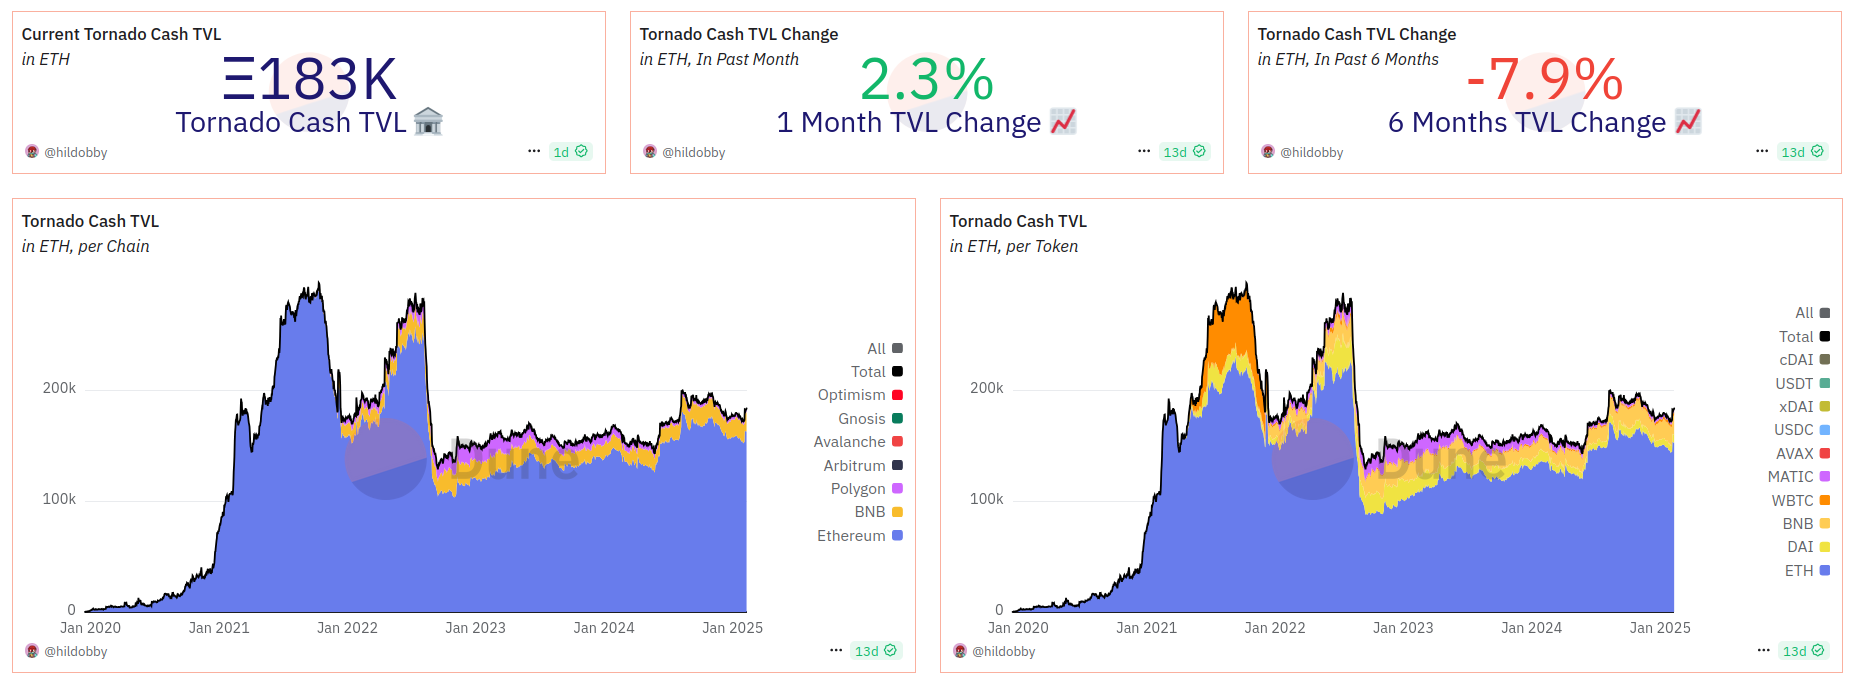
\includegraphics[width=0.95\textwidth]{chapters/imgs/tornadocashdunestatisticstvl.png}  
    \caption{TVL di 183k ETH $\sim$ €456M}
\end{figure}

\begin{figure}[H]
    \centering
    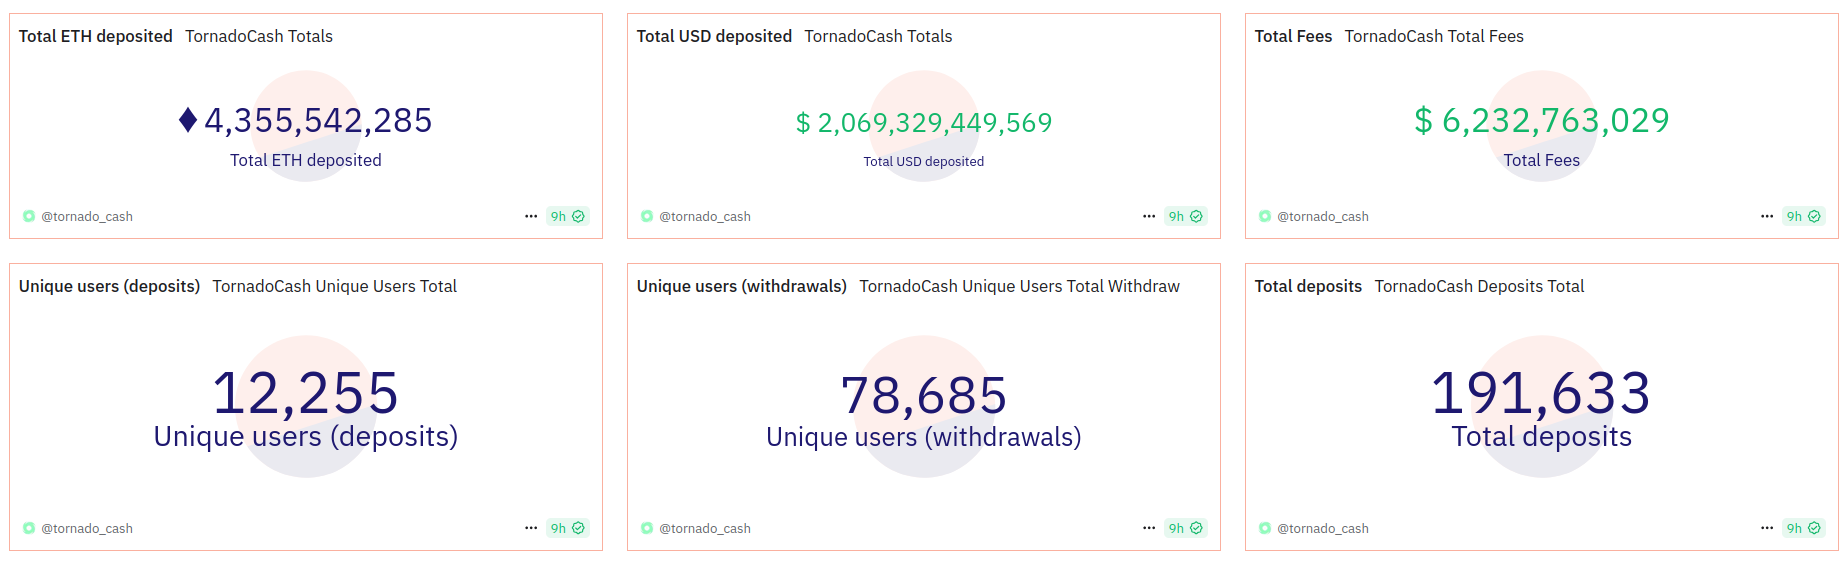
\includegraphics[width=0.95\textwidth]{chapters/imgs/tornadocashdunestatisticsdepositswithdrawals.png}
    \caption{Utilizzo totale fino ad oggi}
\end{figure}

\begin{figure}[H]
    \centering
    \begin{minipage}{0.6\textwidth}
        \centering
        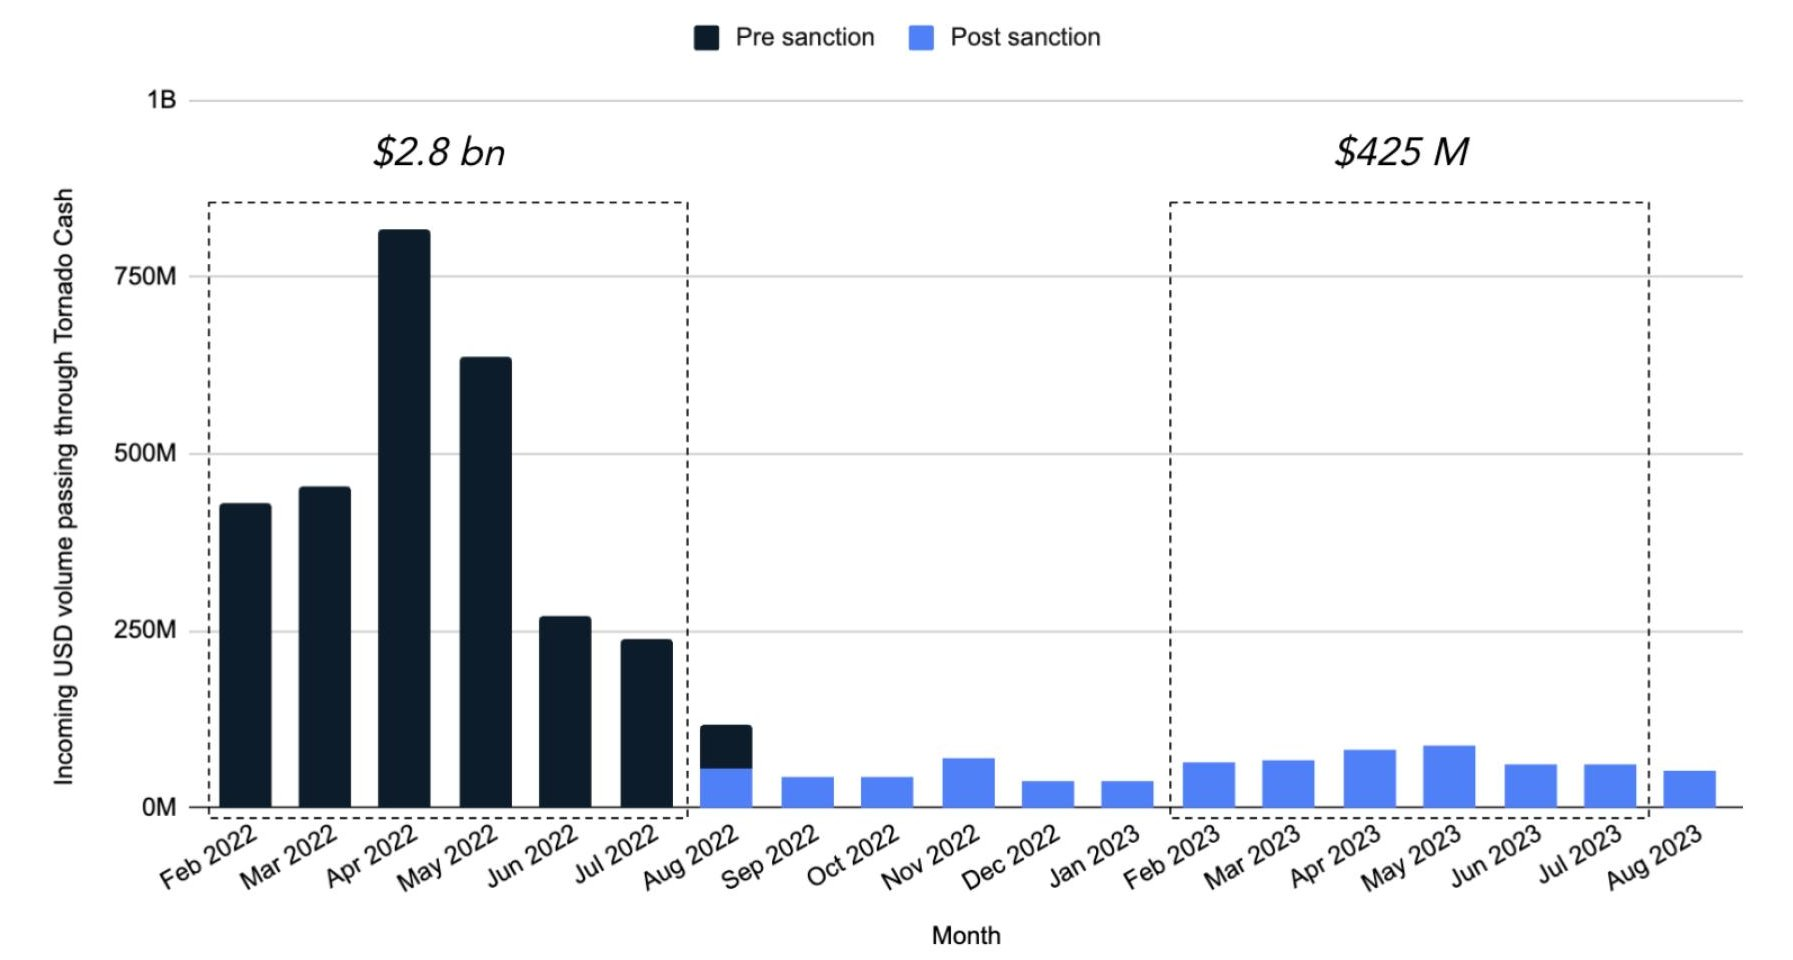
\includegraphics[width=\textwidth]{chapters/imgs/incomingvolpreandpostsanctions.jpg}
    \end{minipage}
    \hspace{0.04\textwidth}
    \begin{minipage}{0.6\textwidth}
        \centering
        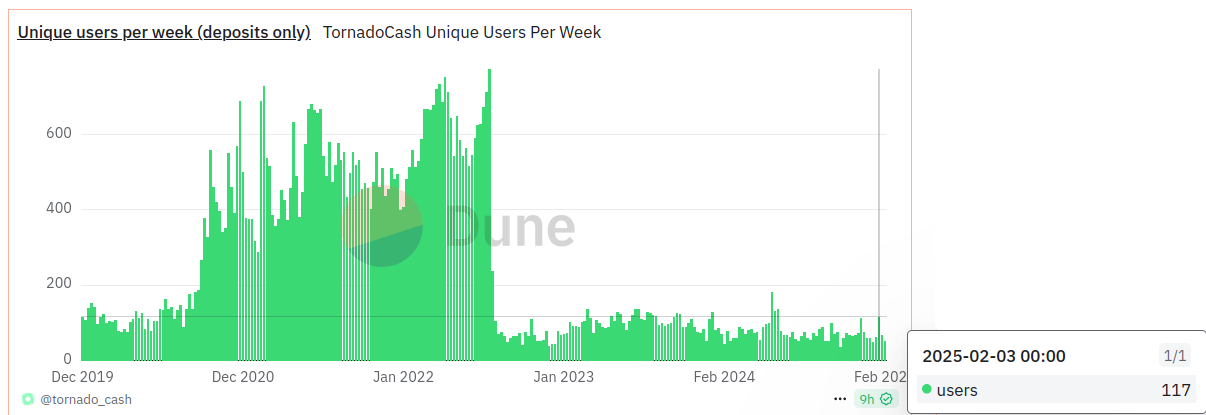
\includegraphics[width=\textwidth]{chapters/imgs/tornadocashdunestatisticsdepositsuniqueperweek.png}
    \end{minipage}
    \caption{Nonostante le sanzioni, è ancora utilizzato}
\end{figure}

\section{Community e sviluppi}
La community di \textit{Tornado Cash} è attiva. Il \href{https://t.me/TornadoCashOfficialDAO/}{nuovo gruppo Telegram ufficiale} è stato istituito tramite la \href{https://etherscan.io/address/0x01f9Db30C7EEaAa81f4037eABEaB22682E9Cc61C#code}{Proposal di governance \#57}, proposta il \textbf{25 novembre 2024}, per contrastare i gruppi scam. Questa proposta è riconosciuta ufficialmente su \textit{CoinMarketCap}\cite{coinmarketcap} e \textit{CoinGecko}\cite{coingecko}, inserendo il link nell'icona di Telegram. Il vecchio account Twitter/X è inattivo, ma la DAO gestisce attivamente il protocollo. Gruppi Telegram con oltre 10k membri sono spesso scam con account inattivi comprati.

\textit{Domanda cruciale}: come vietare codice decentralizzato, come gli smart contract di \textit{Tornado Cash}, che sono eseguiti su macchine virtuali locali? Nonostante le sanzioni degli USA (in corso di revoca e rimozione), \textit{Tornado Cash} resiste, utilizzato da chi cerca privacy in contesti sensibili.